\documentclass{whiteboard}
\begin{document}
\begin{frame}[plain,t]
 \bbcover{OJ 11991}{Easy Problem from Rujia Liu?}{Prof. Edson Alves}{Faculdade UnB Gama}
\end{frame}

\begin{frame}[plain,t]
\vspace*{\fill}
 \bbenglish{``Though Rujia Liu usually sets hard problems for contests (for example, regional contests like Xi’an 2006, Beijing 2007 and Wuhan 2009, or UVa OJ contests like Rujia Liu’s Presents 1 and 2), he occasionally sets easy problem (for example, ‘the Coco-Cola Store’ in UVa OJ), to encourage more people to solve his problems :D''}

 \vspace{0.1in}

 \bbenglish{Given an array, your task is to find the $k$-th occurrence (from left to right) of an integer $v$. To make the problem more difficult (and interesting!), you’ll have to answer $m$ such queries.}
\vspace*{\fill}
\end{frame}

\begin{frame}[plain,t]
\vspace*{\fill}
 \bbtext{``Embora Rujia Liu geralmente crie problemas difíceis para as competições (por exemplo, competições regionais como Xi’an 2006, Beijing 2007 e Wuhan 2009, ou competições do OJ como Rujia Liu’s Presents 1 e 2), de vez em quando ele cria um problema fácil (por exemplo, ‘the Coco-Cola Store’ no OJ), para encorajar mais pessoas a resolverem seus problemas :D''}

 \vspace{0.1in}

 \bbtext{Dado um vetor, sua tarefa é encontrar a $k$-ésima ocorrência (da esquerda para direita) de um inteiro $v$. Para tornar o problema mais difícil (e interessante!), você deverá responder $m$ consultas deste tipo.}
\vspace*{\fill}
\end{frame}

\begin{frame}[plain,t]
\vspace*{\fill}
 \bbbold{Input}

 \vspace{0.1in}

 \bbenglish{There are several test cases. The first line of each test case contains two integers $n, m$ $(1\leq n, m\leq 100,000)$, the number of elements in the array, and the number of queries. The next line contains $n$ positive integers not larger than 1,000,000. Each of the following $m$ lines contains two integer $k$ and $v$ ($1\leq k\leq n, 1\leq v\leq 1,000,000$).  The input is terminated by end-of-file (EOF).}

 \vspace{0.1in}

 \bbbold{Output}

 \vspace{0.1in}

 \bbenglish{For each query, print the $1$-based location of the occurrence. If there is no such element, output ‘\texttt{0}’ instead.}
\vspace*{\fill}
\end{frame}

\begin{frame}[plain,t]
\vspace*{\fill}
 \bbbold{Entrada}

 \vspace{0.1in}

 \bbtext{Há vários casos de teste. A primeira linha de cada caso de teste contém dois inteiros $n, m$ $(1\leq n, m\leq 100,000)$, o número de elementos no vetor e o número de consultas. A próxima linha contém $n$ inteiros positivos menores ou iguais a 1,000,000. Cada uma das $m$ linhas seguintes contém dois inteiros $k$ e $v$ ($1\leq k\leq n, 1\leq v\leq 1,000,000$). A entrada é terminada por fim de arquivo (EOF).}

 \vspace{0.1in}

 \bbbold{Saída}

 \vspace{0.1in}

 \bbtext{Para cada consulta imprima a localização da ocorrência, começando em $1$. Se não existe tal elemento, imprima ‘\texttt{0}’.}
\vspace*{\fill}
\end{frame}

\begin{frame}[plain,t]
\begin{tikzpicture}
\node[draw,opacity=0] at (0, 0) {x};
\node[draw,opacity=0] at (14, 8) {x};
 \node at (0, 7) { \bbbold{Exemplo de entrada e saída} };
 \node at (1, 6) { \bbtext{8} };
 \node at (1.5, 6) { \bbtext{4} };
\end{tikzpicture}
\end{frame}

\begin{frame}[plain,t]
\begin{tikzpicture}
\node[draw,opacity=0] at (0, 0) {x};
\node[draw,opacity=0] at (14, 8) {x};
 \node at (0, 7) { \bbbold{Exemplo de entrada e saída} };
 \node at (1, 6) { \bbtext{8} };
 \node at (1.5, 6) { \bbtext{4} };
 \node at (1, 5) { \footnotesize \bbcomment{\# de elementos} };
 \node[anchor=west] at (2.4, 6) { \footnotesize \bbcomment{\# de consultas} };
 \draw[->,color=BBViolet] (1, 5.2) -- (1, 5.8);
 \draw[->,color=BBViolet] (2.3, 6) to (1.8, 6);
\end{tikzpicture}
\end{frame}

\begin{frame}[plain,t]
\begin{tikzpicture}
\node[draw,opacity=0] at (0, 0) {x};
\node[draw,opacity=0] at (14, 8) {x};
 \node at (0, 7) { \bbbold{Exemplo de entrada e saída} };
 \node at (1, 6) { \bbtext{8} };
 \node at (1.5, 6) { \bbtext{4} };
 \node at (1, 5) { \bbtext{1} };
 \node at (1.5, 5) { \bbtext{3} };
 \node at (2, 5) { \bbtext{2} };
 \node at (2.5, 5) { \bbtext{2} };
 \node at (3, 5) { \bbtext{4} };
 \node at (3.5, 5) { \bbtext{3} };
 \node at (4, 5) { \bbtext{2} };
 \node at (4.5, 5) { \bbtext{1} };
\end{tikzpicture}
\end{frame}

\begin{frame}[plain,t]
\begin{tikzpicture}
\node[draw,opacity=0] at (0, 0) {x};
\node[draw,opacity=0] at (14, 8) {x};
 \node at (0, 7) { \bbbold{Exemplo de entrada e saída} };
 \node at (1, 6) { \bbtext{8} };
 \node at (1.5, 6) { \bbtext{4} };
 \node at (1, 5) { \bbtext{1} };
 \node at (1.5, 5) { \bbtext{3} };
 \node at (2, 5) { \bbtext{2} };
 \node at (2.5, 5) { \bbtext{2} };
 \node at (3, 5) { \bbtext{4} };
 \node at (3.5, 5) { \bbtext{3} };
 \node at (4, 5) { \bbtext{2} };
 \node at (4.5, 5) { \bbtext{1} };
 \node[anchor=west] at (5, 5) { \footnotesize \bbcomment{elementos} };
 \draw[->,color=BBViolet] (5.0, 5) to (4.7, 5);
\end{tikzpicture}
\end{frame}

\begin{frame}[plain,t]
\begin{tikzpicture}
\node[draw,opacity=0] at (0, 0) {x};
\node[draw,opacity=0] at (14, 8) {x};
 \node at (0, 7) { \bbbold{Exemplo de entrada e saída} };
 \node at (1, 6) { \bbtext{8} };
 \node at (1.5, 6) { \bbtext{4} };
 \node at (1, 5) { \bbtext{1} };
 \node at (1.5, 5) { \bbtext{3} };
 \node at (2, 5) { \bbtext{2} };
 \node at (2.5, 5) { \bbtext{2} };
 \node at (3, 5) { \bbtext{4} };
 \node at (3.5, 5) { \bbtext{3} };
 \node at (4, 5) { \bbtext{2} };
 \node at (4.5, 5) { \bbtext{1} };
 \node at (1, 4) { \bbtext{1} };
 \node at (1.5, 4) { \bbtext{3} };
\end{tikzpicture}
\end{frame}

\begin{frame}[plain,t]
\begin{tikzpicture}
\node[draw,opacity=0] at (0, 0) {x};
\node[draw,opacity=0] at (14, 8) {x};
 \node at (0, 7) { \bbbold{Exemplo de entrada e saída} };
 \node at (1, 6) { \bbtext{8} };
 \node at (1.5, 6) { \bbtext{4} };
 \node at (1, 5) { \bbtext{1} };
 \node at (1.5, 5) { \bbtext{3} };
 \node at (2, 5) { \bbtext{2} };
 \node at (2.5, 5) { \bbtext{2} };
 \node at (3, 5) { \bbtext{4} };
 \node at (3.5, 5) { \bbtext{3} };
 \node at (4, 5) { \bbtext{2} };
 \node at (4.5, 5) { \bbtext{1} };
 \node at (1, 4) { \bbtext{1} };
 \node at (1.5, 4) { \bbtext{3} };
 \node at (1, 3) { \footnotesize \bbcomment{primeira ocorrência} };
 \node[anchor=west] at (2.4, 4) { \footnotesize \bbcomment{do elemento 3} };
 \draw[->,color=BBViolet] (1, 3.2) -- (1, 3.8);
 \draw[->,color=BBViolet] (2.3, 4) to (1.8, 4);
\end{tikzpicture}
\end{frame}

\begin{frame}[plain,t]
\begin{tikzpicture}
\node[draw,opacity=0] at (0, 0) {x};
\node[draw,opacity=0] at (14, 8) {x};
 \node at (0, 7) { \bbbold{Exemplo de entrada e saída} };
 \node at (1, 6) { \bbtext{8} };
 \node at (1.5, 6) { \bbtext{4} };
 \node at (1, 5) { \bbtext{1} };
 \node at (1.5, 5) { \bbtext{3} };
 \node at (2, 5) { \bbtext{2} };
 \node at (2.5, 5) { \bbtext{2} };
 \node at (3, 5) { \bbtext{4} };
 \node at (3.5, 5) { \bbtext{3} };
 \node at (4, 5) { \bbtext{2} };
 \node at (4.5, 5) { \bbtext{1} };
 \node at (1, 4) { \bbtext{1} };
 \node at (1.5, 4) { \bbtext{3} };
 \draw[->,color=BBViolet,very thick] (2, 5.5) [bend right] to (1.5, 5.2);
\end{tikzpicture}
\end{frame}

\begin{frame}[plain,t]
\begin{tikzpicture}
\node[draw,opacity=0] at (0, 0) {x};
\node[draw,opacity=0] at (14, 8) {x};
 \node at (0, 7) { \bbbold{Exemplo de entrada e saída} };
 \node at (1, 6) { \bbtext{8} };
 \node at (1.5, 6) { \bbtext{4} };
 \node at (1, 5) { \bbtext{1} };
 \node at (1.5, 5) { \bbtext{3} };
 \node at (2, 5) { \bbtext{2} };
 \node at (2.5, 5) { \bbtext{2} };
 \node at (3, 5) { \bbtext{4} };
 \node at (3.5, 5) { \bbtext{3} };
 \node at (4, 5) { \bbtext{2} };
 \node at (4.5, 5) { \bbtext{1} };
 \node at (1, 4) { \bbtext{1} };
 \node at (1.5, 4) { \bbtext{3} };
 \draw[->,color=BBViolet,very thick] (2, 5.5) [bend right] to (1.5, 5.2);
 \draw[->,color=BBOrange,very thick] (1.8, 4) to (2.4, 4);
 \node[anchor=west] at (2.5, 4) { \bbinfo{2} };
\end{tikzpicture}
\end{frame}

\begin{frame}[plain,t]
\begin{tikzpicture}
\node[draw,opacity=0] at (0, 0) {x};
\node[draw,opacity=0] at (14, 8) {x};
 \node at (0, 7) { \bbbold{Exemplo de entrada e saída} };
 \node at (1, 6) { \bbtext{8} };
 \node at (1.5, 6) { \bbtext{4} };
 \node at (1, 5) { \bbtext{1} };
 \node at (1.5, 5) { \bbtext{3} };
 \node at (2, 5) { \bbtext{2} };
 \node at (2.5, 5) { \bbtext{2} };
 \node at (3, 5) { \bbtext{4} };
 \node at (3.5, 5) { \bbtext{3} };
 \node at (4, 5) { \bbtext{2} };
 \node at (4.5, 5) { \bbtext{1} };
 \node at (1, 4) { \bbtext{1} };
 \node at (1.5, 4) { \bbtext{3} };
 \draw[->,color=BBOrange,very thick] (1.8, 4) to (2.4, 4);
 \node[anchor=west] at (2.5, 4) { \bbinfo{2} };
 \node at (1, 3) { \bbtext{2} };
 \node at (1.5, 3) { \bbtext{4} };
\end{tikzpicture}
\end{frame}

\begin{frame}[plain,t]
\begin{tikzpicture}
\node[draw,opacity=0] at (0, 0) {x};
\node[draw,opacity=0] at (14, 8) {x};
 \node at (0, 7) { \bbbold{Exemplo de entrada e saída} };
 \node at (1, 6) { \bbtext{8} };
 \node at (1.5, 6) { \bbtext{4} };
 \node at (1, 5) { \bbtext{1} };
 \node at (1.5, 5) { \bbtext{3} };
 \node at (2, 5) { \bbtext{2} };
 \node at (2.5, 5) { \bbtext{2} };
 \node at (3, 5) { \bbtext{4} };
 \node at (3.5, 5) { \bbtext{3} };
 \node at (4, 5) { \bbtext{2} };
 \node at (4.5, 5) { \bbtext{1} };
 \node at (1, 4) { \bbtext{1} };
 \node at (1.5, 4) { \bbtext{3} };
 \draw[->,color=BBOrange,very thick] (1.8, 4) to (2.4, 4);
 \node[anchor=west] at (2.5, 4) { \bbinfo{2} };
 \node at (1, 3) { \bbtext{2} };
 \node at (1.5, 3) { \bbtext{4} };
 \node at (1, 2) { \footnotesize \bbcomment{segunda ocorrência} };
 \node[anchor=west] at (2.4, 3) { \footnotesize \bbcomment{do elemento 4} };
 \draw[->,color=BBViolet] (1, 2.2) -- (1, 2.8);
 \draw[->,color=BBViolet] (2.3, 3) to (1.8, 3);
\end{tikzpicture}
\end{frame}

\begin{frame}[plain,t]
\begin{tikzpicture}
\node[draw,opacity=0] at (0, 0) {x};
\node[draw,opacity=0] at (14, 8) {x};
 \node at (0, 7) { \bbbold{Exemplo de entrada e saída} };
 \node at (1, 6) { \bbtext{8} };
 \node at (1.5, 6) { \bbtext{4} };
 \node at (1, 5) { \bbtext{1} };
 \node at (1.5, 5) { \bbtext{3} };
 \node at (2, 5) { \bbtext{2} };
 \node at (2.5, 5) { \bbtext{2} };
 \node at (3, 5) { \bbtext{4} };
 \node at (3.5, 5) { \bbtext{3} };
 \node at (4, 5) { \bbtext{2} };
 \node at (4.5, 5) { \bbtext{1} };
 \node at (1, 4) { \bbtext{1} };
 \node at (1.5, 4) { \bbtext{3} };
 \draw[->,color=BBOrange,very thick] (1.8, 4) to (2.4, 4);
 \node[anchor=west] at (2.5, 4) { \bbinfo{2} };
 \node at (1, 3) { \bbtext{2} };
 \node at (1.5, 3) { \bbtext{4} };
 \draw[->,color=BBOrange,very thick] (1.8, 3) to (2.4, 3);
 \node[anchor=west] at (2.5, 3) { \bbinfo{0} };
\end{tikzpicture}
\end{frame}

\begin{frame}[plain,t]
\begin{tikzpicture}
\node[draw,opacity=0] at (0, 0) {x};
\node[draw,opacity=0] at (14, 8) {x};
 \node at (0, 7) { \bbbold{Exemplo de entrada e saída} };
 \node at (1, 6) { \bbtext{8} };
 \node at (1.5, 6) { \bbtext{4} };
 \node at (1, 5) { \bbtext{1} };
 \node at (1.5, 5) { \bbtext{3} };
 \node at (2, 5) { \bbtext{2} };
 \node at (2.5, 5) { \bbtext{2} };
 \node at (3, 5) { \bbtext{4} };
 \node at (3.5, 5) { \bbtext{3} };
 \node at (4, 5) { \bbtext{2} };
 \node at (4.5, 5) { \bbtext{1} };
 \node at (1, 4) { \bbtext{1} };
 \node at (1.5, 4) { \bbtext{3} };
 \draw[->,color=BBOrange,very thick] (1.8, 4) to (2.4, 4);
 \node[anchor=west] at (2.5, 4) { \bbinfo{2} };
 \node at (1, 3) { \bbtext{2} };
 \node at (1.5, 3) { \bbtext{4} };
 \draw[->,color=BBOrange,very thick] (1.8, 3) to (2.4, 3);
 \node[anchor=west] at (2.5, 3) { \bbinfo{0} };
 \node at (1, 2) { \bbtext{3} };
 \node at (1.5, 2) { \bbtext{2} };
\end{tikzpicture}
\end{frame}

\begin{frame}[plain,t]
\begin{tikzpicture}
\node[draw,opacity=0] at (0, 0) {x};
\node[draw,opacity=0] at (14, 8) {x};
 \node at (0, 7) { \bbbold{Exemplo de entrada e saída} };
 \node at (1, 6) { \bbtext{8} };
 \node at (1.5, 6) { \bbtext{4} };
 \node at (1, 5) { \bbtext{1} };
 \node at (1.5, 5) { \bbtext{3} };
 \node at (2, 5) { \bbtext{2} };
 \node at (2.5, 5) { \bbtext{2} };
 \node at (3, 5) { \bbtext{4} };
 \node at (3.5, 5) { \bbtext{3} };
 \node at (4, 5) { \bbtext{2} };
 \node at (4.5, 5) { \bbtext{1} };
 \node at (1, 4) { \bbtext{1} };
 \node at (1.5, 4) { \bbtext{3} };
 \draw[->,color=BBOrange,very thick] (1.8, 4) to (2.4, 4);
 \node[anchor=west] at (2.5, 4) { \bbinfo{2} };
 \node at (1, 3) { \bbtext{2} };
 \node at (1.5, 3) { \bbtext{4} };
 \draw[->,color=BBOrange,very thick] (1.8, 3) to (2.4, 3);
 \node[anchor=west] at (2.5, 3) { \bbinfo{0} };
 \node at (1, 2) { \bbtext{3} };
 \node at (1.5, 2) { \bbtext{2} };
 \draw[->,color=BBViolet,very thick] (4.5, 5.5) [bend right] to (4, 5.2);
\end{tikzpicture}
\end{frame}

\begin{frame}[plain,t]
\begin{tikzpicture}
\node[draw,opacity=0] at (0, 0) {x};
\node[draw,opacity=0] at (14, 8) {x};
 \node at (0, 7) { \bbbold{Exemplo de entrada e saída} };
 \node at (1, 6) { \bbtext{8} };
 \node at (1.5, 6) { \bbtext{4} };
 \node at (1, 5) { \bbtext{1} };
 \node at (1.5, 5) { \bbtext{3} };
 \node at (2, 5) { \bbtext{2} };
 \node at (2.5, 5) { \bbtext{2} };
 \node at (3, 5) { \bbtext{4} };
 \node at (3.5, 5) { \bbtext{3} };
 \node at (4, 5) { \bbtext{2} };
 \node at (4.5, 5) { \bbtext{1} };
 \node at (1, 4) { \bbtext{1} };
 \node at (1.5, 4) { \bbtext{3} };
 \draw[->,color=BBOrange,very thick] (1.8, 4) to (2.4, 4);
 \node[anchor=west] at (2.5, 4) { \bbinfo{2} };
 \node at (1, 3) { \bbtext{2} };
 \node at (1.5, 3) { \bbtext{4} };
 \draw[->,color=BBOrange,very thick] (1.8, 3) to (2.4, 3);
 \node[anchor=west] at (2.5, 3) { \bbinfo{0} };
 \node at (1, 2) { \bbtext{3} };
 \node at (1.5, 2) { \bbtext{2} };
 \draw[->,color=BBViolet,very thick] (4.5, 5.5) [bend right] to (4, 5.2);
 \draw[->,color=BBOrange,very thick] (1.8, 2) to (2.4, 2);
 \node[anchor=west] at (2.5, 2) { \bbinfo{7} };
\end{tikzpicture}
\end{frame}

\begin{frame}[plain,t]
\begin{tikzpicture}
\node[draw,opacity=0] at (0, 0) {x};
\node[draw,opacity=0] at (14, 8) {x};
 \node at (0, 7) { \bbbold{Exemplo de entrada e saída} };
 \node at (1, 6) { \bbtext{8} };
 \node at (1.5, 6) { \bbtext{4} };
 \node at (1, 5) { \bbtext{1} };
 \node at (1.5, 5) { \bbtext{3} };
 \node at (2, 5) { \bbtext{2} };
 \node at (2.5, 5) { \bbtext{2} };
 \node at (3, 5) { \bbtext{4} };
 \node at (3.5, 5) { \bbtext{3} };
 \node at (4, 5) { \bbtext{2} };
 \node at (4.5, 5) { \bbtext{1} };
 \node at (1, 4) { \bbtext{1} };
 \node at (1.5, 4) { \bbtext{3} };
 \draw[->,color=BBOrange,very thick] (1.8, 4) to (2.4, 4);
 \node[anchor=west] at (2.5, 4) { \bbinfo{2} };
 \node at (1, 3) { \bbtext{2} };
 \node at (1.5, 3) { \bbtext{4} };
 \draw[->,color=BBOrange,very thick] (1.8, 3) to (2.4, 3);
 \node[anchor=west] at (2.5, 3) { \bbinfo{0} };
 \node at (1, 2) { \bbtext{3} };
 \node at (1.5, 2) { \bbtext{2} };
 \draw[->,color=BBOrange,very thick] (1.8, 2) to (2.4, 2);
 \node[anchor=west] at (2.5, 2) { \bbinfo{7} };
 \node at (1, 1) { \bbtext{4} };
 \node at (1.5, 1) { \bbtext{2} };
\end{tikzpicture}
\end{frame}

\begin{frame}[plain,t]
\begin{tikzpicture}
\node[draw,opacity=0] at (0, 0) {x};
\node[draw,opacity=0] at (14, 8) {x};
 \node at (0, 7) { \bbbold{Exemplo de entrada e saída} };
 \node at (1, 6) { \bbtext{8} };
 \node at (1.5, 6) { \bbtext{4} };
 \node at (1, 5) { \bbtext{1} };
 \node at (1.5, 5) { \bbtext{3} };
 \node at (2, 5) { \bbtext{2} };
 \node at (2.5, 5) { \bbtext{2} };
 \node at (3, 5) { \bbtext{4} };
 \node at (3.5, 5) { \bbtext{3} };
 \node at (4, 5) { \bbtext{2} };
 \node at (4.5, 5) { \bbtext{1} };
 \node at (1, 4) { \bbtext{1} };
 \node at (1.5, 4) { \bbtext{3} };
 \draw[->,color=BBOrange,very thick] (1.8, 4) to (2.4, 4);
 \node[anchor=west] at (2.5, 4) { \bbinfo{2} };
 \node at (1, 3) { \bbtext{2} };
 \node at (1.5, 3) { \bbtext{4} };
 \draw[->,color=BBOrange,very thick] (1.8, 3) to (2.4, 3);
 \node[anchor=west] at (2.5, 3) { \bbinfo{0} };
 \node at (1, 2) { \bbtext{3} };
 \node at (1.5, 2) { \bbtext{2} };
 \draw[->,color=BBOrange,very thick] (1.8, 2) to (2.4, 2);
 \node[anchor=west] at (2.5, 2) { \bbinfo{7} };
 \node at (1, 1) { \bbtext{4} };
 \node at (1.5, 1) { \bbtext{2} };
 \draw[->,color=BBOrange,very thick] (1.8, 1) to (2.4, 1);
 \node[anchor=west] at (2.5, 1) { \bbinfo{0} };
\end{tikzpicture}
\end{frame}

\begin{frame}[plain,t]
\begin{tikzpicture}
\node[draw,opacity=0] at (0, 0) {x};
\node[draw,opacity=0] at (14, 8) {x};
 \node at (0, 7) { \bbbold{Solução} };
\end{tikzpicture}
\end{frame}

\begin{frame}[plain,t]
\begin{tikzpicture}
\node[draw,opacity=0] at (0, 0) {x};
\node[draw,opacity=0] at (14, 8) {x};
 \node at (0, 7) { \bbbold{Solução} };
 \node[draw,circle,very thick] (A1) at (1, 5) { \bbtext{1} };
 \node[draw,circle,very thick] (A2) at (2, 5) { \bbtext{2} };
 \node[draw,circle,very thick] (A3) at (3, 5) { \bbtext{3} };
 \node[draw,circle,very thick] (A4) at (4, 5) { \bbtext{4} };
 \node[draw,circle,very thick] (A5) at (5, 5) { \bbtext{5} };
 \node[draw,circle,very thick] (A6) at (6, 5) { \bbtext{6} };
 \node[draw,circle,very thick] (A7) at (7, 5) { \bbtext{7} };
 \node[draw,circle,very thick] (A8) at (8, 5) { \bbtext{8} };
 \node[draw,circle,very thick] (B1) at (1, 2) { $x_1$ };
 \node[draw,circle,very thick] (B2) at (2, 2) { $x_2$ };
 \node[draw,circle,very thick] (B3) at (3, 2) { $x_3$ };
 \node[draw,circle,very thick] (B4) at (4, 2) { $x_4$ };
 \node[draw,circle,very thick] (B5) at (5, 2) { $x_5$ };
 \node[draw,circle,very thick] (B6) at (6, 2) { $x_6$ };
 \node[draw,circle,very thick] (B7) at (7, 2) { $x_7$ };
 \node[draw,circle,very thick] (B8) at (8, 2) { $x_8$ };
\end{tikzpicture}
\end{frame}

\begin{frame}[plain,t]
\begin{tikzpicture}
\node[draw,opacity=0] at (0, 0) {x};
\node[draw,opacity=0] at (14, 8) {x};
 \node at (0, 7) { \bbbold{Solução} };
 \node[draw,circle,very thick] (A1) at (1, 5) { \bbtext{1} };
 \node[draw,circle,very thick] (A2) at (2, 5) { \bbtext{2} };
 \node[draw,circle,very thick] (A3) at (3, 5) { \bbtext{3} };
 \node[draw,circle,very thick] (A4) at (4, 5) { \bbtext{4} };
 \node[draw,circle,very thick] (A5) at (5, 5) { \bbtext{5} };
 \node[draw,circle,very thick] (A6) at (6, 5) { \bbtext{6} };
 \node[draw,circle,very thick] (A7) at (7, 5) { \bbtext{7} };
 \node[draw,circle,very thick] (A8) at (8, 5) { \bbtext{8} };
 \node[draw,circle,very thick] (B1) at (1.5, 2) { $1$ };
 \node[draw,circle,very thick] (B2) at (3.5, 2) { $2$ };
 \node[draw,circle,very thick] (B3) at (5.5, 2) { $3$ };
 \node[draw,circle,very thick] (B4) at (7.5, 2) { $4$ };
\end{tikzpicture}
\end{frame}

\begin{frame}[plain,t]
\begin{tikzpicture}
\node[draw,opacity=0] at (0, 0) {x};
\node[draw,opacity=0] at (14, 8) {x};
 \node at (0, 7) { \bbbold{Solução} };
 \node[draw,circle,very thick] (A1) at (1, 5) { \bbtext{1} };
 \node[draw,circle,very thick] (A2) at (2, 5) { \bbtext{2} };
 \node[draw,circle,very thick] (A3) at (3, 5) { \bbtext{3} };
 \node[draw,circle,very thick] (A4) at (4, 5) { \bbtext{4} };
 \node[draw,circle,very thick] (A5) at (5, 5) { \bbtext{5} };
 \node[draw,circle,very thick] (A6) at (6, 5) { \bbtext{6} };
 \node[draw,circle,very thick] (A7) at (7, 5) { \bbtext{7} };
 \node[draw,circle,very thick] (A8) at (8, 5) { \bbtext{8} };
 \node[draw,circle,very thick] (B1) at (1.5, 2) { $1$ };
 \node[draw,circle,very thick] (B2) at (3.5, 2) { $2$ };
 \node[draw,circle,very thick] (B3) at (5.5, 2) { $3$ };
 \node[draw,circle,very thick] (B4) at (7.5, 2) { $4$ };
 \draw[-latex,very thick] (B1) to (A1);
 \draw[-latex,very thick] (B1) to (A8);
\end{tikzpicture}
\end{frame}

\begin{frame}[plain,t]
\begin{tikzpicture}
\node[draw,opacity=0] at (0, 0) {x};
\node[draw,opacity=0] at (14, 8) {x};
 \node at (0, 7) { \bbbold{Solução} };
 \node[draw,circle,very thick] (A1) at (1, 5) { \bbtext{1} };
 \node[draw,circle,very thick] (A2) at (2, 5) { \bbtext{2} };
 \node[draw,circle,very thick] (A3) at (3, 5) { \bbtext{3} };
 \node[draw,circle,very thick] (A4) at (4, 5) { \bbtext{4} };
 \node[draw,circle,very thick] (A5) at (5, 5) { \bbtext{5} };
 \node[draw,circle,very thick] (A6) at (6, 5) { \bbtext{6} };
 \node[draw,circle,very thick] (A7) at (7, 5) { \bbtext{7} };
 \node[draw,circle,very thick] (A8) at (8, 5) { \bbtext{8} };
 \node[draw,circle,very thick] (B1) at (1.5, 2) { $1$ };
 \node[draw,circle,very thick] (B2) at (3.5, 2) { $2$ };
 \node[draw,circle,very thick] (B3) at (5.5, 2) { $3$ };
 \node[draw,circle,very thick] (B4) at (7.5, 2) { $4$ };
 \draw[-latex,very thick] (B1) to (A1);
 \draw[-latex,very thick] (B1) to (A8);
 \draw[-latex,very thick] (B2) to (A3);
 \draw[-latex,very thick] (B2) to (A4);
 \draw[-latex,very thick] (B2) to (A7);
\end{tikzpicture}
\end{frame}

\begin{frame}[plain,t]
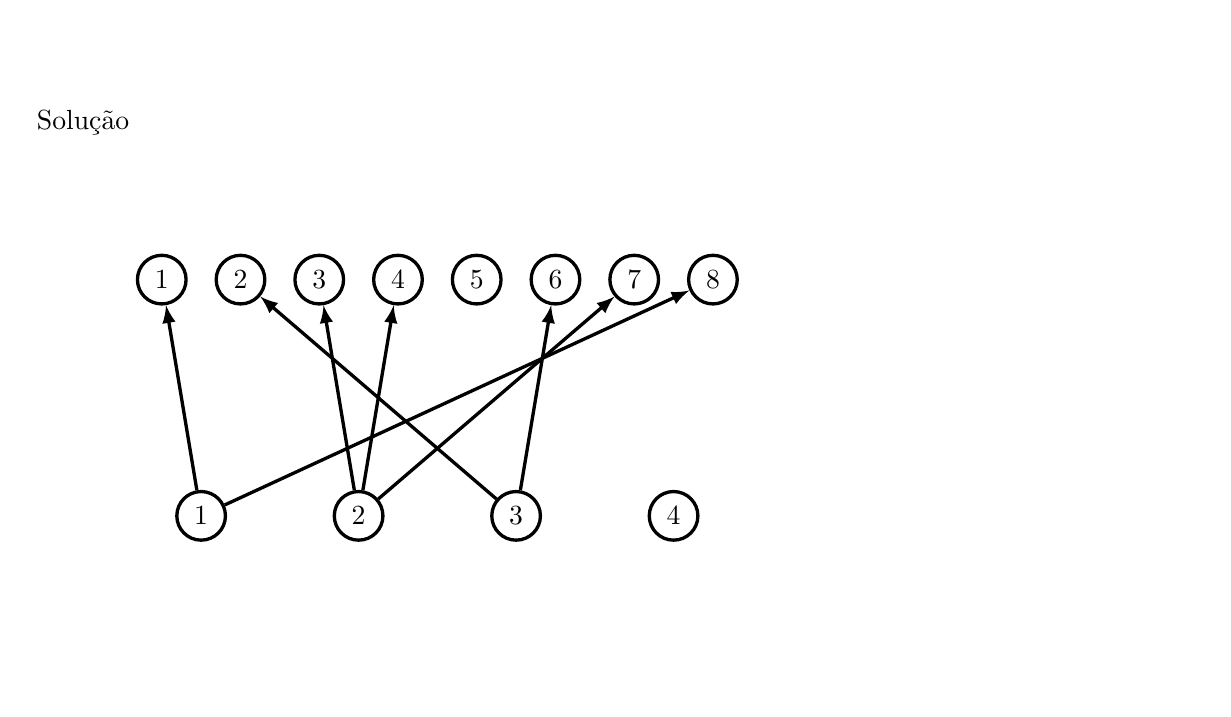
\begin{tikzpicture}
\node[draw,opacity=0] at (0, 0) {x};
\node[draw,opacity=0] at (14, 8) {x};
 \node at (0, 7) { \bbbold{Solução} };
 \node[draw,circle,very thick] (A1) at (1, 5) { \bbtext{1} };
 \node[draw,circle,very thick] (A2) at (2, 5) { \bbtext{2} };
 \node[draw,circle,very thick] (A3) at (3, 5) { \bbtext{3} };
 \node[draw,circle,very thick] (A4) at (4, 5) { \bbtext{4} };
 \node[draw,circle,very thick] (A5) at (5, 5) { \bbtext{5} };
 \node[draw,circle,very thick] (A6) at (6, 5) { \bbtext{6} };
 \node[draw,circle,very thick] (A7) at (7, 5) { \bbtext{7} };
 \node[draw,circle,very thick] (A8) at (8, 5) { \bbtext{8} };
 \node[draw,circle,very thick] (B1) at (1.5, 2) { $1$ };
 \node[draw,circle,very thick] (B2) at (3.5, 2) { $2$ };
 \node[draw,circle,very thick] (B3) at (5.5, 2) { $3$ };
 \node[draw,circle,very thick] (B4) at (7.5, 2) { $4$ };
 \draw[-latex,very thick] (B1) to (A1);
 \draw[-latex,very thick] (B1) to (A8);
 \draw[-latex,very thick] (B2) to (A3);
 \draw[-latex,very thick] (B2) to (A4);
 \draw[-latex,very thick] (B2) to (A7);
 \draw[-latex,very thick] (B3) to (A2);
 \draw[-latex,very thick] (B3) to (A6);
\end{tikzpicture}
\end{frame}

\begin{frame}[plain,t]
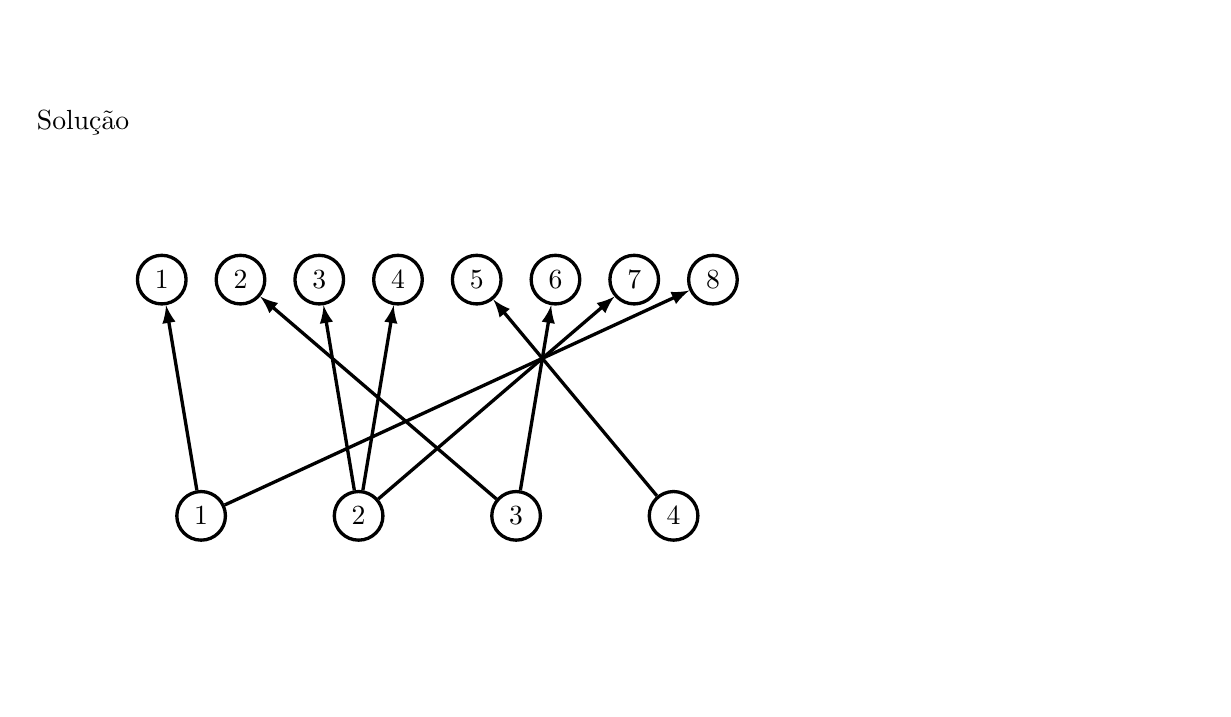
\begin{tikzpicture}
\node[draw,opacity=0] at (0, 0) {x};
\node[draw,opacity=0] at (14, 8) {x};
 \node at (0, 7) { \bbbold{Solução} };
 \node[draw,circle,very thick] (A1) at (1, 5) { \bbtext{1} };
 \node[draw,circle,very thick] (A2) at (2, 5) { \bbtext{2} };
 \node[draw,circle,very thick] (A3) at (3, 5) { \bbtext{3} };
 \node[draw,circle,very thick] (A4) at (4, 5) { \bbtext{4} };
 \node[draw,circle,very thick] (A5) at (5, 5) { \bbtext{5} };
 \node[draw,circle,very thick] (A6) at (6, 5) { \bbtext{6} };
 \node[draw,circle,very thick] (A7) at (7, 5) { \bbtext{7} };
 \node[draw,circle,very thick] (A8) at (8, 5) { \bbtext{8} };
 \node[draw,circle,very thick] (B1) at (1.5, 2) { $1$ };
 \node[draw,circle,very thick] (B2) at (3.5, 2) { $2$ };
 \node[draw,circle,very thick] (B3) at (5.5, 2) { $3$ };
 \node[draw,circle,very thick] (B4) at (7.5, 2) { $4$ };
 \draw[-latex,very thick] (B1) to (A1);
 \draw[-latex,very thick] (B1) to (A8);
 \draw[-latex,very thick] (B2) to (A3);
 \draw[-latex,very thick] (B2) to (A4);
 \draw[-latex,very thick] (B2) to (A7);
 \draw[-latex,very thick] (B3) to (A2);
 \draw[-latex,very thick] (B3) to (A6);
 \draw[-latex,very thick] (B4) to (A5);
\end{tikzpicture}
\end{frame}

\begin{frame}[plain,t]
\begin{tikzpicture}
\node[draw,opacity=0] at (0, 0) {x};
\node[draw,opacity=0] at (14, 8) {x};
 \node at (0, 7) { \bbbold{Solução} };
 \node[draw,circle,very thick] (A1) at (1, 5) { \bbtext{1} };
 \node[draw,circle,very thick] (A2) at (2, 5) { \bbtext{2} };
 \node[draw,circle,very thick] (A3) at (3, 5) { \bbtext{3} };
 \node[draw,circle,very thick] (A4) at (4, 5) { \bbtext{4} };
 \node[draw,circle,very thick] (A5) at (5, 5) { \bbtext{5} };
 \node[draw,circle,very thick] (A6) at (6, 5) { \bbtext{6} };
 \node[draw,circle,very thick] (A7) at (7, 5) { \bbtext{7} };
 \node[draw,circle,very thick] (A8) at (8, 5) { \bbtext{8} };
 \node[draw,circle,very thick] (B1) at (1.5, 2) { $1$ };
 \node[draw,circle,very thick] (B2) at (3.5, 2) { $2$ };
 \node[draw,circle,very thick] (B3) at (5.5, 2) { $3$ };
 \node[draw,circle,very thick] (B4) at (7.5, 2) { $4$ };
 \draw[-latex,very thick] (B1) to (A1);
 \draw[-latex,very thick] (B1) to (A8);
 \draw[-latex,very thick] (B2) to (A3);
 \draw[-latex,very thick] (B2) to (A4);
 \draw[-latex,very thick] (B2) to (A7);
 \draw[-latex,very thick] (B3) to (A2);
 \draw[-latex,very thick] (B3) to (A6);
 \draw[-latex,very thick] (B4) to (A5);
 \draw[very thick] (11, 5.5) to (11, 1.5);
 \node at (10.5, 5) { $1$ };
 \node at (10.5, 4) { $2$ };
 \node at (10.5, 3) { $3$ };
 \node at (10.5, 2) { $4$ };
 \node[anchor=west] at (8, 6) { \footnotesize \bbcomment{Lista de adjacências} };
 \draw[->,color=BBViolet] (10, 5.8) to (10.8, 5.6);
\end{tikzpicture}
\end{frame}

\begin{frame}[plain,t]
\begin{tikzpicture}
\node[draw,opacity=0] at (0, 0) {x};
\node[draw,opacity=0] at (14, 8) {x};
 \node at (0, 7) { \bbbold{Solução} };
 \node[draw,circle,very thick] (A1) at (1, 5) { \bbtext{1} };
 \node[draw,circle,very thick] (A2) at (2, 5) { \bbtext{2} };
 \node[draw,circle,very thick] (A3) at (3, 5) { \bbtext{3} };
 \node[draw,circle,very thick] (A4) at (4, 5) { \bbtext{4} };
 \node[draw,circle,very thick] (A5) at (5, 5) { \bbtext{5} };
 \node[draw,circle,very thick] (A6) at (6, 5) { \bbtext{6} };
 \node[draw,circle,very thick] (A7) at (7, 5) { \bbtext{7} };
 \node[draw,circle,very thick] (A8) at (8, 5) { \bbtext{8} };
 \node[draw,circle,very thick] (B1) at (1.5, 2) { $1$ };
 \node[draw,circle,very thick] (B2) at (3.5, 2) { $2$ };
 \node[draw,circle,very thick] (B3) at (5.5, 2) { $3$ };
 \node[draw,circle,very thick] (B4) at (7.5, 2) { $4$ };
 \draw[-latex,very thick] (B1) to (A1);
 \draw[-latex,very thick] (B1) to (A8);
 \draw[-latex,very thick] (B2) to (A3);
 \draw[-latex,very thick] (B2) to (A4);
 \draw[-latex,very thick] (B2) to (A7);
 \draw[-latex,very thick] (B3) to (A2);
 \draw[-latex,very thick] (B3) to (A6);
 \draw[-latex,very thick] (B4) to (A5);
 \draw[very thick] (11, 5.5) to (11, 1.5);
 \node at (10.5, 5) { $1$ };
 \node at (10.5, 4) { $2$ };
 \node at (10.5, 3) { $3$ };
 \node at (10.5, 2) { $4$ };
 \node[anchor=west] at (8, 6) { \footnotesize \bbcomment{Lista de adjacências} };
 \draw[->,color=BBViolet] (10, 5.8) to (10.8, 5.6);
 \node at (11.5, 5) { \bbinfo{1} };
 \node at (12, 5) { \bbinfo{8} };
\end{tikzpicture}
\end{frame}

\begin{frame}[plain,t]
\begin{tikzpicture}
\node[draw,opacity=0] at (0, 0) {x};
\node[draw,opacity=0] at (14, 8) {x};
 \node at (0, 7) { \bbbold{Solução} };
 \node[draw,circle,very thick] (A1) at (1, 5) { \bbtext{1} };
 \node[draw,circle,very thick] (A2) at (2, 5) { \bbtext{2} };
 \node[draw,circle,very thick] (A3) at (3, 5) { \bbtext{3} };
 \node[draw,circle,very thick] (A4) at (4, 5) { \bbtext{4} };
 \node[draw,circle,very thick] (A5) at (5, 5) { \bbtext{5} };
 \node[draw,circle,very thick] (A6) at (6, 5) { \bbtext{6} };
 \node[draw,circle,very thick] (A7) at (7, 5) { \bbtext{7} };
 \node[draw,circle,very thick] (A8) at (8, 5) { \bbtext{8} };
 \node[draw,circle,very thick] (B1) at (1.5, 2) { $1$ };
 \node[draw,circle,very thick] (B2) at (3.5, 2) { $2$ };
 \node[draw,circle,very thick] (B3) at (5.5, 2) { $3$ };
 \node[draw,circle,very thick] (B4) at (7.5, 2) { $4$ };
 \draw[-latex,very thick] (B1) to (A1);
 \draw[-latex,very thick] (B1) to (A8);
 \draw[-latex,very thick] (B2) to (A3);
 \draw[-latex,very thick] (B2) to (A4);
 \draw[-latex,very thick] (B2) to (A7);
 \draw[-latex,very thick] (B3) to (A2);
 \draw[-latex,very thick] (B3) to (A6);
 \draw[-latex,very thick] (B4) to (A5);
 \draw[very thick] (11, 5.5) to (11, 1.5);
 \node at (10.5, 5) { $1$ };
 \node at (10.5, 4) { $2$ };
 \node at (10.5, 3) { $3$ };
 \node at (10.5, 2) { $4$ };
 \node[anchor=west] at (8, 6) { \footnotesize \bbcomment{Lista de adjacências} };
 \draw[->,color=BBViolet] (10, 5.8) to (10.8, 5.6);
 \node at (11.5, 5) { \bbinfo{1} };
 \node at (12, 5) { \bbinfo{8} };
 \node at (11.5, 4) { \bbinfo{3} };
 \node at (12.0, 4) { \bbinfo{4} };
 \node at (12.5, 4) { \bbinfo{7} };
\end{tikzpicture}
\end{frame}

\begin{frame}[plain,t]
\begin{tikzpicture}
\node[draw,opacity=0] at (0, 0) {x};
\node[draw,opacity=0] at (14, 8) {x};
 \node at (0, 7) { \bbbold{Solução} };
 \node[draw,circle,very thick] (A1) at (1, 5) { \bbtext{1} };
 \node[draw,circle,very thick] (A2) at (2, 5) { \bbtext{2} };
 \node[draw,circle,very thick] (A3) at (3, 5) { \bbtext{3} };
 \node[draw,circle,very thick] (A4) at (4, 5) { \bbtext{4} };
 \node[draw,circle,very thick] (A5) at (5, 5) { \bbtext{5} };
 \node[draw,circle,very thick] (A6) at (6, 5) { \bbtext{6} };
 \node[draw,circle,very thick] (A7) at (7, 5) { \bbtext{7} };
 \node[draw,circle,very thick] (A8) at (8, 5) { \bbtext{8} };
 \node[draw,circle,very thick] (B1) at (1.5, 2) { $1$ };
 \node[draw,circle,very thick] (B2) at (3.5, 2) { $2$ };
 \node[draw,circle,very thick] (B3) at (5.5, 2) { $3$ };
 \node[draw,circle,very thick] (B4) at (7.5, 2) { $4$ };
 \draw[-latex,very thick] (B1) to (A1);
 \draw[-latex,very thick] (B1) to (A8);
 \draw[-latex,very thick] (B2) to (A3);
 \draw[-latex,very thick] (B2) to (A4);
 \draw[-latex,very thick] (B2) to (A7);
 \draw[-latex,very thick] (B3) to (A2);
 \draw[-latex,very thick] (B3) to (A6);
 \draw[-latex,very thick] (B4) to (A5);
 \draw[very thick] (11, 5.5) to (11, 1.5);
 \node at (10.5, 5) { $1$ };
 \node at (10.5, 4) { $2$ };
 \node at (10.5, 3) { $3$ };
 \node at (10.5, 2) { $4$ };
 \node[anchor=west] at (8, 6) { \footnotesize \bbcomment{Lista de adjacências} };
 \draw[->,color=BBViolet] (10, 5.8) to (10.8, 5.6);
 \node at (11.5, 5) { \bbinfo{1} };
 \node at (12, 5) { \bbinfo{8} };
 \node at (11.5, 4) { \bbinfo{3} };
 \node at (12.0, 4) { \bbinfo{4} };
 \node at (12.5, 4) { \bbinfo{7} };
 \node at (11.5, 3) { \bbinfo{2} };
 \node at (12.0, 3) { \bbinfo{6} };
\end{tikzpicture}
\end{frame}

\begin{frame}[plain,t]
\begin{tikzpicture}
\node[draw,opacity=0] at (0, 0) {x};
\node[draw,opacity=0] at (14, 8) {x};
 \node at (0, 7) { \bbbold{Solução} };
 \node[draw,circle,very thick] (A1) at (1, 5) { \bbtext{1} };
 \node[draw,circle,very thick] (A2) at (2, 5) { \bbtext{2} };
 \node[draw,circle,very thick] (A3) at (3, 5) { \bbtext{3} };
 \node[draw,circle,very thick] (A4) at (4, 5) { \bbtext{4} };
 \node[draw,circle,very thick] (A5) at (5, 5) { \bbtext{5} };
 \node[draw,circle,very thick] (A6) at (6, 5) { \bbtext{6} };
 \node[draw,circle,very thick] (A7) at (7, 5) { \bbtext{7} };
 \node[draw,circle,very thick] (A8) at (8, 5) { \bbtext{8} };
 \node[draw,circle,very thick] (B1) at (1.5, 2) { $1$ };
 \node[draw,circle,very thick] (B2) at (3.5, 2) { $2$ };
 \node[draw,circle,very thick] (B3) at (5.5, 2) { $3$ };
 \node[draw,circle,very thick] (B4) at (7.5, 2) { $4$ };
 \draw[-latex,very thick] (B1) to (A1);
 \draw[-latex,very thick] (B1) to (A8);
 \draw[-latex,very thick] (B2) to (A3);
 \draw[-latex,very thick] (B2) to (A4);
 \draw[-latex,very thick] (B2) to (A7);
 \draw[-latex,very thick] (B3) to (A2);
 \draw[-latex,very thick] (B3) to (A6);
 \draw[-latex,very thick] (B4) to (A5);
 \draw[very thick] (11, 5.5) to (11, 1.5);
 \node at (10.5, 5) { $1$ };
 \node at (10.5, 4) { $2$ };
 \node at (10.5, 3) { $3$ };
 \node at (10.5, 2) { $4$ };
 \node[anchor=west] at (8, 6) { \footnotesize \bbcomment{Lista de adjacências} };
 \draw[->,color=BBViolet] (10, 5.8) to (10.8, 5.6);
 \node at (11.5, 5) { \bbinfo{1} };
 \node at (12, 5) { \bbinfo{8} };
 \node at (11.5, 4) { \bbinfo{3} };
 \node at (12.0, 4) { \bbinfo{4} };
 \node at (12.5, 4) { \bbinfo{7} };
 \node at (11.5, 3) { \bbinfo{2} };
 \node at (12.0, 3) { \bbinfo{6} };
 \node at (11.5, 2) { \bbinfo{5} };
\end{tikzpicture}
\end{frame}

\begin{frame}[plain,t]
\begin{tikzpicture}
\node[draw,opacity=0] at (0, 0) {x};
\node[draw,opacity=0] at (14, 8) {x};
 \node at (0, 7) { \bbbold{Solução} };
 \node[draw,circle,very thick] (A1) at (1, 5) { \bbtext{1} };
 \node[draw,circle,very thick] (A2) at (2, 5) { \bbtext{2} };
 \node[draw,circle,very thick] (A3) at (3, 5) { \bbtext{3} };
 \node[draw,circle,very thick] (A4) at (4, 5) { \bbtext{4} };
 \node[draw,circle,very thick] (A5) at (5, 5) { \bbtext{5} };
 \node[draw,circle,very thick] (A6) at (6, 5) { \bbtext{6} };
 \node[draw,circle,very thick] (A7) at (7, 5) { \bbtext{7} };
 \node[draw,circle,very thick] (A8) at (8, 5) { \bbtext{8} };
 \node[draw,circle,very thick] (B1) at (1.5, 2) { $1$ };
 \node[draw,circle,very thick] (B2) at (3.5, 2) { $2$ };
 \node[draw,circle,very thick] (B3) at (5.5, 2) { $3$ };
 \node[draw,circle,very thick] (B4) at (7.5, 2) { $4$ };
 \draw[-latex,very thick] (B1) to (A1);
 \draw[-latex,very thick] (B1) to (A8);
 \draw[-latex,very thick] (B2) to (A3);
 \draw[-latex,very thick] (B2) to (A4);
 \draw[-latex,very thick] (B2) to (A7);
 \draw[-latex,very thick] (B3) to (A2);
 \draw[-latex,very thick] (B3) to (A6);
 \draw[-latex,very thick] (B4) to (A5);
 \draw[very thick] (11, 5.5) to (11, 1.5);
 \node at (10.5, 5) { $1$ };
 \node at (10.5, 4) { $2$ };
 \node at (10.5, 3) { $3$ };
 \node at (10.5, 2) { $4$ };
 \node[anchor=west] at (8, 6) { \footnotesize \bbcomment{Lista de adjacências} };
 \draw[->,color=BBViolet] (10, 5.8) to (10.8, 5.6);
 \node at (11.5, 5) { \bbinfo{1} };
 \node at (12, 5) { \bbinfo{8} };
 \node at (11.5, 4) { \bbinfo{3} };
 \node at (12.0, 4) { \bbinfo{4} };
 \node at (12.5, 4) { \bbinfo{7} };
 \node at (11.5, 3) { \bbinfo{2} };
 \node at (12.0, 3) { \bbinfo{6} };
 \node at (11.5, 2) { \bbinfo{5} };
 \node[anchor=west] at (9, 1) { \footnotesize \bbcomment{Consultas em $O(1)$} };
 \draw[->,color=BBViolet] (10.3, 1.2) to (10.8, 1.4);
\end{tikzpicture}
\end{frame}

\begin{frame}[plain,t]
 \inputsnippet{cpp}{1}{18}{codes/11991.cpp}
\end{frame}

\begin{frame}[plain,t]
 \inputsnippet{cpp}{19}{36}{codes/11991.cpp}
\end{frame}

\begin{frame}[plain,t]
 \inputsnippet{cpp}{37}{54}{codes/11991.cpp}
\end{frame}

\end{document}
